\section{Entities and How to Represent Them}

``An entity is an object or concept in the real world that can be distinctly identified''~\cite{entityorientedsearch2018}.
Typical examples of entities include ``John Smith'', ``Google Inc.'', ``Rome'', which correspond to a person, an organization, and a location, respectively. These are all \emph{named entities}, i.e., entities that can be identified by a proper noun.
In practise, however, \acl{nlp} tools also recognize more general \emph{concepts}, such as dates (e.g., ``June 20, 2025''), monetary values (e.g., ``100\,\$''), quantities (e.g., ``5 kilograms''), or other abstract objects (e.g., gravity, emotion)~\cite{muc6_overview_1995}.
This occurs because, at the implementation level, the same methods can detect both named entities and concepts~\cite{entityorientedsearch2018}. Modern natural language toolkits, such as spaCy~\cite{honnibal2020spacy}, flair~\cite{akbik2019flair}, or Stanford CoreNLP~\cite{manning-EtAl:2014:P14-5}, provide models capable of extracting both types of entities~\cite{spacy-ner-labels,flair-ner-ontonotes,stanfordnlp-ner}. For this reason, throughout this thesis, we use the term \emph{entity} to refer to both named entities and concepts, as formalized in the following definition, which is based on \textcite{entityorientedsearch2018} definition:
\begin{definition}[Entity]
An \emph{entity} is a uniquely identifiable object, thing, or concept. 
It is described through a set of \emph{entity properties}, always including 
at least one unique identifier and one name (which may in some cases coincide). 
Additinal entity properties include types, attributes, and 
relationships to other entities or concepts.
\end{definition}

For example, consider the entity \textsc{Barack Obama}. 
A possible unique identifier is ``Barack Obama (44th US president)'', which can serve also as a name, alongwith ``Barack Obama.'' 
The entity belongs to the types \texttt{Person} and \texttt{Politician}. 
Its attributes include the full birth name ``Barack Hussein Obama II'' and the date of birth ``Aug 4, 1961''. 
Relationships connect this entity to other entities such as its birthplace, \textsc{Honolulu}, and its spouse, \textsc{Michelle Obama}.

Entities can be stored and maintained in a \emph{\acl{kr}} or a \emph{\acl{kb}}~\cite{entityorientedsearch2018}.
%
\begin{definition}[\Acl{kr}]
A \acf{kr} is a structured or semi-structured collection of entities~\cite{entityorientedsearch2018}.
\end{definition}

Wikipedia~\cite{wikipedia} is a well-known semi-structured \acl{kr}, where each entity is represented as an article (e.g., https://en.wikipedia.org/wiki/Barack\_Obama) containing text semi-structured in different sections, as well as pictures and hyperlinks connected to other entities, similarly to relationships.

While semi-structured repositories are well suited for human consumption, machines require more formalized representations. The \Acl{sw} community has been working to extend the \acs{web} into a machine-interpretable form~\cite{entityorientedsearch2018,decker_sw_rdf_xml_roles_2000}. This effort led to the development of the \acl{sw} stack, encompassing standards such as URIs, XML, \acs{rdf}, SPARQL~\cite{prudhommeaux2008sparql}, and ontology languages like RDFS and OWL~\cite{entityorientedsearch2018}.

The \acf{rdf}~\cite{klyne2004rdf} data model allows to represent an entity as a set of assertions or \emph{facts} about that entity. In this work, we will use \emph{fact} independenlty from the \ac{rdf} syntax, according to the following definition.
\begin{definition}[Fact]
    A fact is an atomic statement, a single and indivisible assertion of a specific piece of information about the world, typically describing a property of an entity or a relationship between entities.
\end{definition}
Example of facts are ``Barack Obama was born on Aug 04, 1961.'' or ``Barack Obama was born in Honolulu.''
Instead, in \ac{rdf} resources are represented as structured triples composed of subject, predicate, and object. The subject and predicate are usually IRIs (Internationalized Resource Identifier~\cite{durst2005iri}---sequences of unicode characters that uniquely identify resources), while the object is usually either a IRI or a literal (used for values such as strings, numbers, and dates, annotated with a datatype and eventually with a language tag)~\cite{klyne2004rdf}.
%
The previous facts appear as follows in \ac{rdf}:
%
\begin{lstlisting}
    <*@\url{http://dbpedia.org/resource/Barack_Obama}@*>
            <*@\url{http://dbpedia.org/ontology/birthName}@*>
                    "Barack Hussein Obama II"@en .

    <*@\url{http://dbpedia.org/resource/Barack_Obama}@*>
            <*@\url{http://dbpedia.org/ontology/birthPlace}@*>
                    <*@\url{http://dbpedia.org/resource/Honolulu}@*> .
\end{lstlisting}

\begin{figure}[h]
\centering
% as of aug 25, 2025
\begin{lstlisting}[style=rdfstyle,caption={Excerpt from the DBpedia~\cite{dbpedia,dbpedia_auer_nucleus_2007} knowledge base entry of \textsc{Barack Obama}, in Turtle format~\cite{prudhommeaux2014turtle}.},label={lis:obama}]
@prefix dbr: <http://dbpedia.org/resource/> .
@prefix dbo: <http://dbpedia.org/ontology/> .
@prefix rdf: <http://www.w3.org/1999/02/22-rdf-syntax-ns#> .
@prefix rdfs: <http://www.w3.org/2000/01/rdf-schema#> .
@prefix xsd: <http://www.w3.org/2001/XMLSchema#> .

dbr:Barack_Obama

        dbo:birthName       "Barack Hussein Obama II"@en ;
        dbo:birthPlace      dbr:Honolulu ;
        dbo:birthDate       "1961-08-04"^^xsd:date ;
        rdf:type            dbo:Person ;
        rdf:type            dbo:Politician ;
        dbo:spouse          dbr:Michelle_Obama ;
        rdfs:comment        "Barack Hussein Obama II ([...] born August 4,
                            1961) is an American politician who served as
                            the 44th president of the United States from
                            2009 to 2017. [...] Obama was the first
                            African-American president [...]"@en .

\end{lstlisting}
\end{figure}

\Cref{lis:obama} shows some \emph{entity properties} for the entity \textsc{Barack Obama} from DBpedia~\cite{dbpedia_auer_nucleus_2007}. It uses \ac{rdf} following the Turtle~\cite{prudhommeaux2014turtle} syntax and includes types (``dbo:Person'', ``dbo:Politician''), attributes (``dbo:birthName'', ``dbo:birthDate'', ``rdfs:comment''), and relationships with other entities (``dbo:birthPlace'', ``dbo:spouse''). Prefixes are defined to avoid repetitive long IRIs.

Structured entity knowledge, such as represented in \ac{rdf}, is usually stored in a \emph{knowledge base}.
%
\todo{intrduce facts and triples and then move to the kb definition}
% kb definition knowledge base definition
\todo{add operation that make a kb. querying, updating, reasoning,...?}
\begin{definition}[\Acl{kb}]
    A \acf{kb}, or a \acf{kg}, is a structured form of \acl{kr} that organizes and stores facts about entities. 
    These facts are typically represented using data models such as \ac{rdf}~\cite{entityorientedsearch2018}.
    %
    When the primary interest lies in the connections between entities, a \acl{kb} is often referred to as a \emph{\acl{kg}}.
\end{definition}
\Cref{fig:barack_kg} shows an example \acl{kg} about \textsc{Barack Obama} and some connected entities.

\begin{figure}[htbp]
    \centering
    % Include the PDF file
    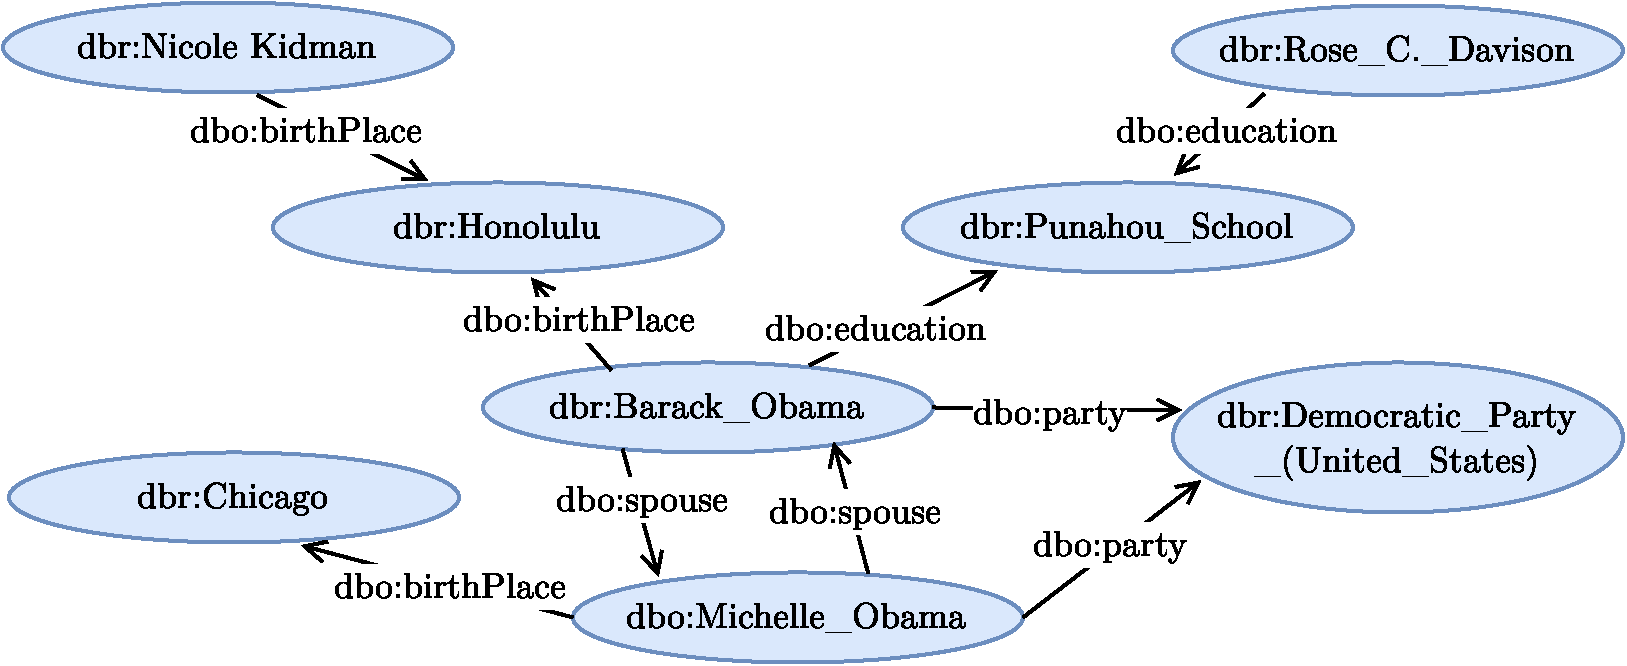
\includegraphics[width=\textwidth]{images/barack_kg.pdf}
    \caption{Example of \acl{kg}. \ac{rdf} prefixes are defined in \Cref{lis:obama}}
    \label{fig:barack_kg}
\end{figure}



\todo{problem of incompleteness. to introduce the incremental kbp. structured means higher quality. unstructured more information lower quality. how is wikidata curated? and dbpedia? to justify the additional human effort. cerca motivazione da paper di hybrid qa come humaniq.}

\subsection{Structured or Unstructured? The Web versus Knowledge Bases}
\todo{can be expanded and called properties of Kbs}
%
Structured \aclp{kb} are incomplete~\cite{west_kb_completion_2014,entityorientedsearch2018}: for example, as of 2014, 71\% of the people represented in Freebase~\cite{freebase_2008} lacked a recorded place of birth~\cite{west_kb_completion_2014}.
This incompleteness is further supported by several research proposals for questions answering---the task of answering natural language questions (see \todo{})---that have focused on combining the high-quality, machine-readable but low-coverage knowledge from \acp{kb} with the vast amount of unstructured information available in a less reliable form on the \acs{web}~\cite{sawant_neural_kg_web_2016,west_kb_completion_2014,savenkov_qa_kb_text_2016,PRAMANIK2024100833_uniqorn_qa_kb_text,lehmann2024beyond,zhang-etal-2024-spaghetti_heterogeneus_qa,xin_atomr_heterogeneus_kg_2025}.
%
\todo{maybe useful from balog ``Keeping up
with these changes requires a continuous effort from editors and content managers''}
Semi-structured \aclp{kr}, positioned between structured \acp{kb} and the \acs{web}, suffer---at least partially---from both incompleteness and unreliable information form. Compared to the \ac{web}, they are more structured but less broad and comprehensive. Conversely, relative to \acp{kb}, they cover a wider range of information but present it in a less structured and less reliable form.\todo{missing citation? but it is based on previous statements, so probably not needed. maybe I can cite balog but does not say this clearly.}

\Ac{kb} incompleteness also derives from the constant changes intrinsic to the information, e.g., the US president needs to be updated periodically, people can change residency even more frequently, and novel information is constantly produced, for instance, a new movie just announced. Keeping a \ac{kb} up to date demands ongoing effort from editors and content managers~\cite{entityorientedsearch2018}.

While not enforced by definition, real-world \acp{kb} (such as Wikidata~\cite{wikidata,vrandevcic2014wikidata}) and also unstructured \ac{kr} (Wikipedia~\cite{wikipedia}) support \emph{CRUD} operations (Create, Read, Update, Delete)~\cite{elmasri2014fundamentals} to allow their maintenance over time~\cite{shafee2023ten_rules_editing_wikidata}. These operations are also defined in the SPARQL/Update~\cite{seaborne2008sparqlupdate} language.



% \subsection{Information Extraction and Knowledge Base Population}
\todo{not sure where to put this. it is like combining kbs and the web}
\todo{maybe introduce a bit nlp with the objective and computational linguistics with the objective of capturing the meaning of text}

Capturing the meaning of text is a central goal of \acl{nlp}~\cite{entityorientedsearch2018},\todo{say something more about nlp} and the automatic extraction of semantic information from text---such as mentions of named entities, relationships, and attributes---is known as \emph{\acl{ie}}. This has been the objective of major competitions, including the Message Understanding Conference (MUC)~\cite{muc_lessons_1998,muc6_overview_1995,muc7_overview_1998}, the Computational Natural Language Learning (CoNLL) 2003 shared task~\cite{conll2003}, and the Automatic Content Extraction (ACE) program~\cite{ace_2004}.

% Combining the higher-quality information from \ac{kb} with the broader coverage of unstructured data has motivated the research in \emph{\acl{ie}} since three decades ago~\cite{infoextraction2008,entityorientedsearch2018}.
\begin{definition}[Information Extraction]
``\Acf{ie} refers to the automatic extraction of structured information such as entities, relationships between entities, and attributes describing entities from unstructured sources''~\cite{infoextraction2008}.
\end{definition}
The use of \ac{ie} techniques is generally aimed at either \emph{\acl{sta}} or \emph{\acl{kbp}}~\cite{entityorientedsearch2018}.
In the former case, annotating text with information from a \ac{kb} enriches the text with additional semantics, enabling advanced information access functionalities, such as entity-based search and filtering via faceting~\cite{entityorientedsearch2018}.
In the latter case, \ac{ie} is used to populate or update a \ac{kb} with information extracted from unstructured sources to enhance the \ac{kb}'s coverage and keep it up to date.